%% Template for a preprint Letter or Article for submission
%% to the journal Nature.
%% Written by Peter Czoschke, 26 February 2004
%%

\documentclass[%
%superscriptaddress,
%groupedaddress,
%unsortedaddress,
%runinaddress,
%frontmatterverbose, 
%preprint,
showpacs,
%preprintnumbers,
%nofootinbib,
%nobibnotes,
%bibnotes,
 amsmath,amssymb,
 aps,
 twocolumn,
 prl,
 reprint,
%pra,
%prb,
%rmp,
%prstab,
%prstper,
floatfix,
]{revtex4-1}

\usepackage{graphicx}% Include figure files
\usepackage{dcolumn}% Align table columns on decimal point
\usepackage{bm}% bold math
%\usepackage{lineno}
\usepackage{color}
\usepackage{acronym}
\usepackage{multirow}
\usepackage{tabularx}
\usepackage{hyperref}
%\addbibresource{references.bib}
%\linenumbers % Commence numbering lines
%\usepackage{hyperref}% add hypertext capabilities
%\usepackage[mathlines]{lineno}% Enable numbering of text and display math
%\linenumbers\relax % Commence numbering lines
\hypersetup{
%--- fill inside borders ---
  colorlinks=true,        % false: boxed links; true: colored links
  linkcolor=black,         % color of internal links
  citecolor=cyan,         % color of links to bibliography
}

%% make sure you have the nature.cls and naturemag.bst files where
%% LaTeX can find them

%\bibliographystyle{authortitle}

%% Notice placement of commas and superscripts and use of &
%% in the author list

%\author{Hunter Gabbard$^{1}$, Ik Siong Heng$^1$, Chris Messenger$^1$, \\
%    Francesco Tonolini$^2$, \& Roderick Murray-Smith$^2$}

%% ----- comment commands for each of us
\newcommand{\chris}[1]{\textbf{\textcolor{green}{CHRIS: #1}}}
\newcommand{\francesco}[1]{\textbf{\textcolor{red}{FRANCESCO: #1}}}
\newcommand{\hunter}[1]{\textbf{\textcolor{blue}{HUNTER: #1}}}
\newcommand{\siong}[1]{\textbf{\textcolor{cyan}{SIONG: #1}}}
\newcommand{\rod}[1]{\textbf{\textcolor{yellow}{ROD: #1}}}

\begin{document}

\preprint{APS/123-QED}

\title{Estimating Bayesian Parameter Estimation Using Conditional Variational Autoencoders}

\author{Hunter Gabbard$^1$}
 \email{Corresponding author: h.gabbard.1@research.gla.ac.uk}
\author{Ik Siong Heng$^1$}
\author{Chris Messenger$^1$}
\author{Francesco Tonolini$^2$}
\author{\& Roderick Murray-Smith$^2$}

\affiliation{
 SUPA, School of Physics and Astronomy$^1$, \\
 School of Computing Science$^2$, \\
 University of Glasgow, \\
 Glasgow G12 8QQ, United Kingdom \\
}

\date{\today}

\maketitle

\acrodef{BBH}[BBH]{binary black hole}
\acrodef{SNR}[SNR]{signal-to-noise ratio}
\acrodef{PSD}[PSD]{power spectral density}
\acrodef{FFT}[FFT]{fast Fourier transform}
\acrodef{CNN}[CNN]{convolutional neural network}
\acrodef{ROC}[ROC]{receiver operator characteristic}

%
% Introductory paragraph describing the content of the letter
%
\textbf{
With the beginning of the Laser Interferometer Gravitational wave Observatory's 
(LIGO) and Virgo's third observation run well under way, we are now in an era 
where gravitational wave (GW) detection is commonplace. As the sensitivity of 
both detectors increases, we will see more many more detections on a weekly 
and even daily basis.  The current method used to estimate the parameters of 
gravitational wave events is done using a form of Bayesian inference. Although 
effective, Bayesian inference is a computationally expensive method which can 
take of order hours to weeks to complete when applied to a single GW event. We 
propose the use of a conditional variational autoencoder (CVAE) as a 
computationally inexpensive alternative to this approach. Here we show that 
a CVAE can return the posterior estimate for any parameter of a detected GW 
event on the order of microseconds, an immense speed-up over current 
inference techniques.}

%
% Set up parameter estimation problem
%
When performing Bayesian GW parameter estimation, we assume that we are given 
some observed waveform which is buried in noise. For this study, we consider 
the noise to be whitened Gaussian noise. Given a noisy waveform, we would like 
to find an optimal procedure for retrieving some finite set of unknown GW parameters \cite{Jaranowski2012}
. Our procedure should be able to give us an accurate estimate 
of the parameters of our observed signal, while also accounting for the uncertainty 
which arises from having multiple noise realizations of our observed data able to 
be mapped to one parameter estimate.

%
% Describe Bayes Theorem
%
According to Bayes Theorem, a posterior for a set of GW parameters can be described 
by the following expression:

\begin{equation}
    p(\theta|x) = \frac{p(x|\theta) * p(\theta)}{p(x)},
\end{equation}

where $p(\theta|x)$ is the probability of the parameters given observed data, 
$p(x|\theta)$ is the probability of the observed data given the parameters, $p(\theta)$ 
is the prior we put on our parameter distribution and $p(x)$ is the probability of our data. 
We typically assume that $p(x)$ is a constant, $1$, which then reduces to the following equation:

\begin{equation}
    p(\theta|x) \propto p(x|\theta) * p(\theta),
\end{equation}

where $p(\theta|x)$ is the posterior, $p(x|\theta)$ is the likelihood and $p(\theta)$ is the prior. 
For this study, we assume that the noise is stationary with zero mean and some constant variance 
in each detector. Small changes in the power spectrum density over time are not considered in this analysis. 

%
% Describe nested sampling algorithm
%
There are several algorithms which may be used to sample from the posterior distribution 
of astrophysical GW source parameters. The algorithm which is used in our studies is 
the nested sampling algorithm. Nested sampling takes a multi-dimensional evidence 
integral calculation (fully marginalized likelihood) and transforms it into a more 
manageable 1-D integral. Where the fully marginalized likelihood is equivalent to taking 
the integral of the likelihood and multiplying it by the prior \cite{1409.7215}.

The first step of the nested sampling algorithm starts by generating an initial 
set of live points made from the prior distribution. The likelihood for each point 
is calculated and the point with the lowest likelihood is removed. The removed sample 
is then replaced with a new sample which has a higher likelihood. This cycle repeats 
itself until a predefined stopping threshold is achieved \cite{1409.7215}
. Samples 
from the posterior may be drawn by randomly selecting from both all current 'live' 
points and all previously removed 'live' points. 

%
% discuss codebase which we use to generate waveforms, sampling frequency, and paramter space
%
The codebase which we use to do our Bayesian analysis is the Bilby inference library \cite{1811.02042}
. For testing, waveforms have a duration of 1 second, sampling frequency 
of 256Hz, fixed right ascension ($\alpha$), declination ($\delta$), inclination angle 
($\theta_j$), spin, luminosity distance, and polarization angle ($\psi$). We allow 3 
parameters to vary: chirp mass, phase and time of coalescence. Our waveform model is 
\texttt{IMRPhenomPv2} with a minimum cutoff frequency of 20Hz. Analysis is done using 
a single detector (H1) which has a power spectrum density derived from the Advanced 
LIGO design sensitivity curves.

%
% Discuss priors that we use
%
The priors we choose for the analysis are all fixed for the parameters which we do not 
allow to vary in our test set. For other parameters, we set a prior on both component masses from 
35 - 50 solar masses, a phase prior of $0 - 2\pi$, distance prior of 1Gpc - 3Gpc, and 
a time of coalesence prior of $1126259642.4 - 1126259642.6$. The nested sampler is run 
using 1000 live points and has a predefined stopping criteria of $0.1$. The sampler takes 
$\mathcal{O}(3 \: \textrm{minutes})$ to converge.

%
% Conclude bilby section
% 
After the sampler has converged, we draw samples and produce a posterior on the 
astrophysical GW source parameters we are trying to estimate, an example of which 
can be seen for one test event in Fig. 
%\ref{fig:bilby_pos_ex}
. We will now investigate 
whether we can reproduce the results seen in Fig. 
%\ref{fig:bilby_pos_ex} 
using our 
proposed machine learning approach (CVAEs). The advantages of which include orders 
of magnitude speed-up in parameter posterior estimation. 

%\begin{figure}
%    \centering
%    \includegraphics[width=\textwidth]{figures/samp_8_corner.png}
%    \caption{Predicted posterior distributions produced by the Bilby 
%    inference library for a test GW event with chirp mass $31.21$, 
%    phase $2.04$ and time of coalescence $1126259642.5$. Three 
%    contours are plotted in the 2D histograms at 1,2 and 3 sigma 
%    credibility intervals. 1D histograms have 1 sigma vertical 
%    confidence intervals plotted as blue dashed lines.}
%    \label{fig:bilby_pos_ex}
%\end{figure}
   

%
% What is an autoencoder?
%
Conditional variational autoencoders are a form of variational autoencoders 
which are conditioned on an observation. The autoencoders from which they 
are derived are typically used 
for problems involving image reconstruction and attempt to reproduce a  
given input. An autoencoder is composed of two neural networks, an encoder 
and a decoder. The encoder network takes as input an image, then converts 
the image into a lower dimensional space, what is also known as the {\it{latent space}}. 
The output of the encoder is then fed as input to the decoder network 
which generates as output a reconstruction of the original input
image to the encoder network. Through training, we hope to learn a latent space which will 
take on the most important properties of the input training samples.  

%
% What is a variational autoencoder?
%
One failing of an autoencoder is that they are only able to return one 
output for any one given input. In order to produce variable outputs for 
one given input, we need to to utilize what is known as a variational autoencoder.
A variational autoencoder is also composed of both an encoder and a decoder network. 
The major difference between a variational autoencoder and an autoencoder is how the 
latent space is produced. In our variational autoender, the mean and the log squared 
of the standard deviation of the output of the encoder is calculated. We then multiply 
the log squared of the standard deviation by a unit Gaussian distribution which is 
of the same dimension as that of the latent space. This is then summed together 
with the mean to produce the latent space $z$. The latent space is given as input 
to the decoder network, which attempts to reconstruct the given input to 
the encoder network. In this study we use fully-connected layers in 
both the decoder and the encoder networks.

%
% How does our 3-network set-up work?
%
For this study, we will use a combination of three networks; two encoder networks (Encoder-1, Encoder-2) 
and one decoder network. The decoder network takes as input a set of latent space 
$z$ predictions from one of the encoder networks. The decoder network samples from 
the posterior by producing prediction on our parameters $x$. Encoder-1 takes as 
input a set of GW signals and produces a latent space vector $z_1$, while encoder-2 
takes as input both a set of GW signals and their associated source parameters 
and produces a another latent space vector $z_2$.

\begin{figure}
    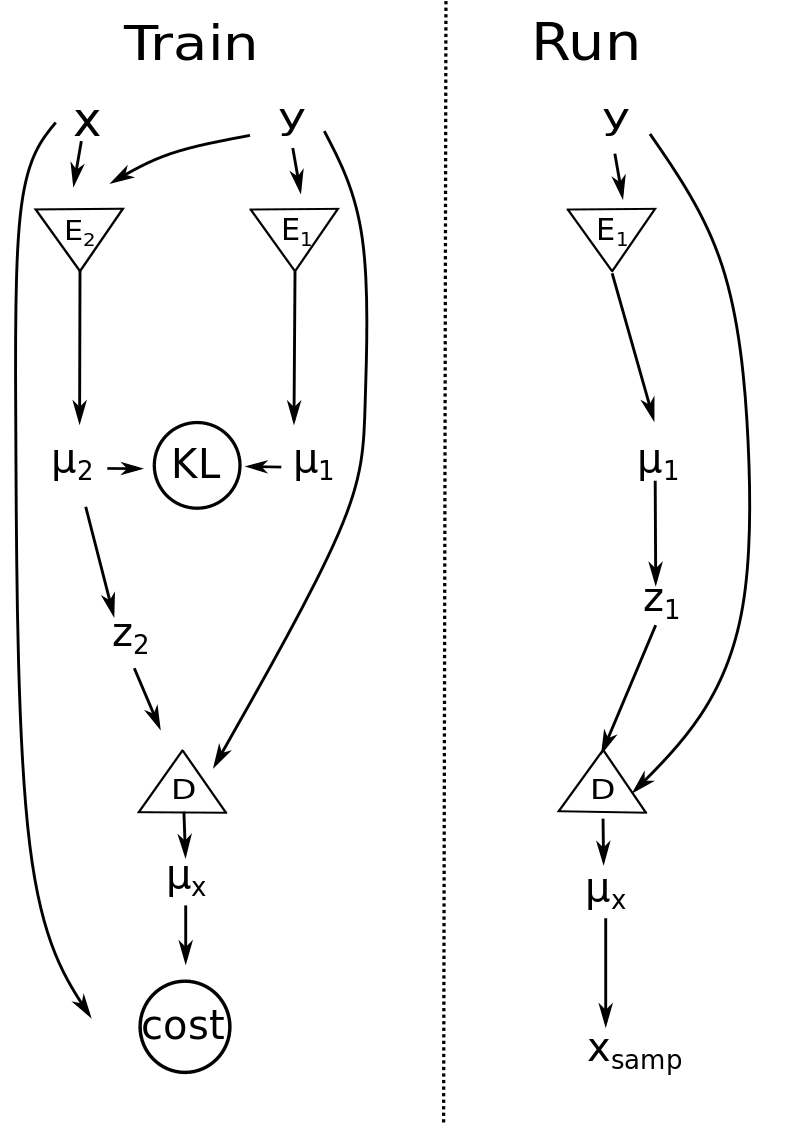
\includegraphics[width=\columnwidth]{images/network_setup.png}
    \caption{\label{fig:network_config} My figure.  An example of a cool figure}
\end{figure}

%
% Training procedure
%
Training is accomplished through a series of 3 steps illustrated in \ref{fig:network_config}. 
In step 1 encoder-1 is given $y_t$ GW training samples and returns as output mean
latent space $z^{y}_{\mu}$. Then in step 2, encoder-2 takes a combination of $(x_{t},y_{t})$ 
and returns $z^{x,y}_{\mu}$. The K-L divergence between both $z^{y}_{\mu}$ and $z^{x,y}_{\mu}$ is 
computed and minimized in order to ensure that both distributions are consistent with each other. 
We finally sample from $z^{x,y}_{\mu}$ using a unitvariant Gaussian distribution 
in order to get a set of $z^{x,y}$ samples. These $z^{x,y}$ samples are combined with 
a set of $y_t$ training samples and fed as input to our decoder network, which attempts 
to reconstruct $x_t$ and outputs a mean predicted $x_{\mu}$. A cost function is then 
computed between $x_{\mu}$ and $x_t$ and is minimized.

%
% Brief introduction to loss functions used in the neural networks
%
In order for our variational autoencoders to learn anything, we need a metric by which 
we can ascertain the effectivness of our networks. This is done by computing 
a loss function which minimizes the difference 
between predictions on the posterior with respect to the truth (cost function) and the Kullback-Leibler divergence 
between latent space distributions $z_1$ and $z_2$. 

%
% Cost function
%
The cost function is constructed by first defining a normalization factor

\begin{equation}
    f_{\textrm{norm}} = 0.5 \cdot \log(c + \exp(x_{\sigma})) - 0.5 \cdot \log(2\pi),
\end{equation}

where $c$ is a small constant and $x_{\sigma}$ are standard deviation predictions 
on the source paramters from the decoder network given latent space predictions 
from encoder-2 ($z_2$) and training GW sigals ($y_{t}$). We then 
compute 

\begin{equation}
    x_{\textrm{diff}} = (x^{z,y}_{\mu} - x_{\textrm{train}})^{2},
\end{equation}

where $x^{z,y}_{\mu}$ are the predicted mean parameters from the decoder network 
and $x_{\textrm{train}}$ are the true training parameters we are 
trying to predict. A Gaussian likelihood is computed and summed over

\begin{equation}
    \textrm{cost} = - \sum (-\frac{x_{\textrm{diff}}}{2c \cdot 
    x^{z^{x,y_{train}}_{\sigma},y_{train}}_{\sigma^{2}}} + f_{\textrm{norm}}),\label{eq:cost}
\end{equation}

where $x^{z^{x,y_{train}}_{\sigma},y_{train}}_{\sigma^{2}}$ are standard deviation squared predictions from the 
decoder network.


%
% KL divergence
%
The purpose of computing the K-L distribution is to train 
encoder-1 and encoder-2 to produce consistant latent space 
distributions. This is done by computing 

\begin{equation}
    \textrm{KL-div} = \sum(\log{z^{y}_{\sigma}}-\log{z^{x,y}_{\sigma}}
    +\frac{\exp{(\log{z^{x,y}_{\sigma^{2}}+c)}}+(z^{x,y}_{\mu}-z^{y}_{\mu})^{2}}{2*\exp{(z^{y}_{\sigma^{2}}})}
    -\frac{1}{2}),\label{eq:kl}
\end{equation}

The mean of the summation in equation \ref{eq:cost}, $\overline{\textrm{cost}}$, 
is then summed together with the mean of the summation in equation \ref{eq:kl}, 
$\overline{\textrm{KL-div}}$ to 
get our final loss function

\begin{equation}
    \textrm{loss} = \overline{\textrm{KL-div}} + \overline{\textrm{cost}}.
\end{equation}

This is loss is then backpropogated through all three networks 
(encoder-1, encoder-2, decoder) and repeated per batch of 
training samples for a pre-defined number of iterations.

%
% loss plot
%
\begin{figure}
    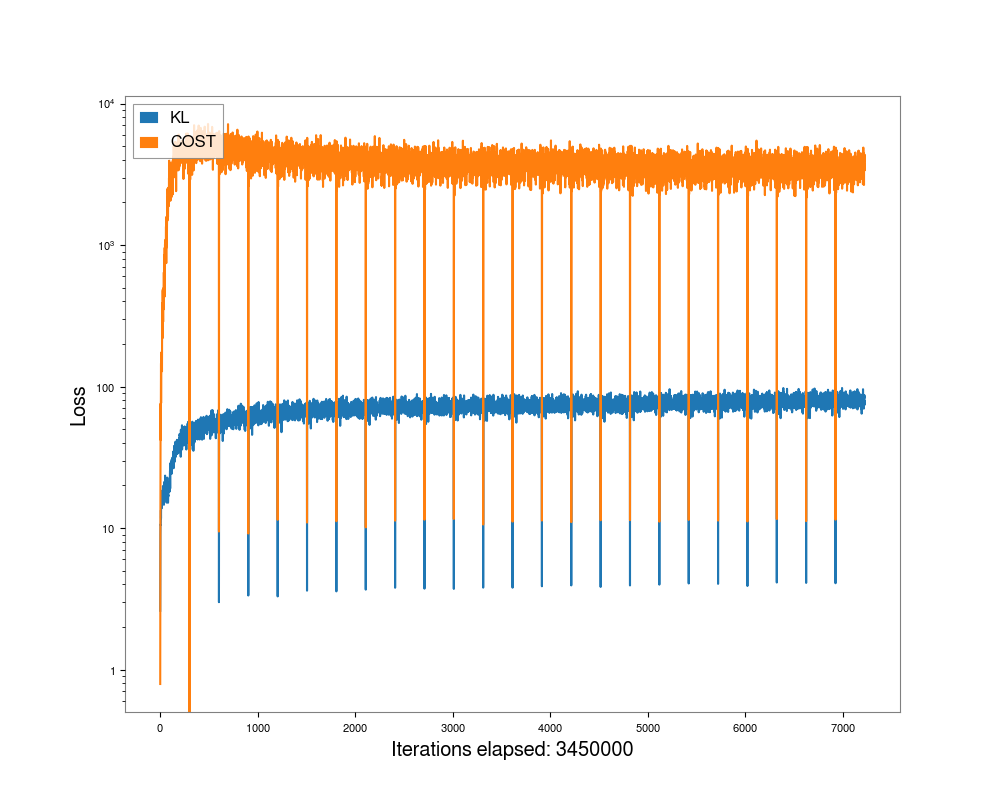
\includegraphics[width=\columnwidth]{images/losses_logscale.png}
    \caption{\label{fig:loss_log} Loss plot with the cost, KL, 
    and total loss values plotted as a function of the total 
    number of training iterations. }
\end{figure}

%
% Test procedure
%
After training has completed, we simply feed encoder-1 our test 
GW signals $y_{test}$. We take the output from encoder-1 $z^{y}_{\mu}$ 
and sample from a univariant Gaussian distribution in order to get 
a set of $z^{y}$ samples. Our $z^{y}$ samples are then combined with our 
test GW signals $y_{test}$ and fed as input to our pre-trained decoder 
network. The decoder network returns a set of mean $x_{\mu}$ predictions 
from which we sample from a Gaussian distribution in order to get 
our final posterior samples.

%
% Results
%
We present results from $25$ test cases of GWs produced from 
a parameter space which is consistent with the prior assumptions  
on the parameter space defined previously. The only difference 
being that all time of coalescence parameters are fixed 
at $0.5s$ within the $1s$ time window. We compare our 
VAE predictions with posteriors produced by the Bilby
inference library.

%
% K-L divergence results
%
\begin{figure}
    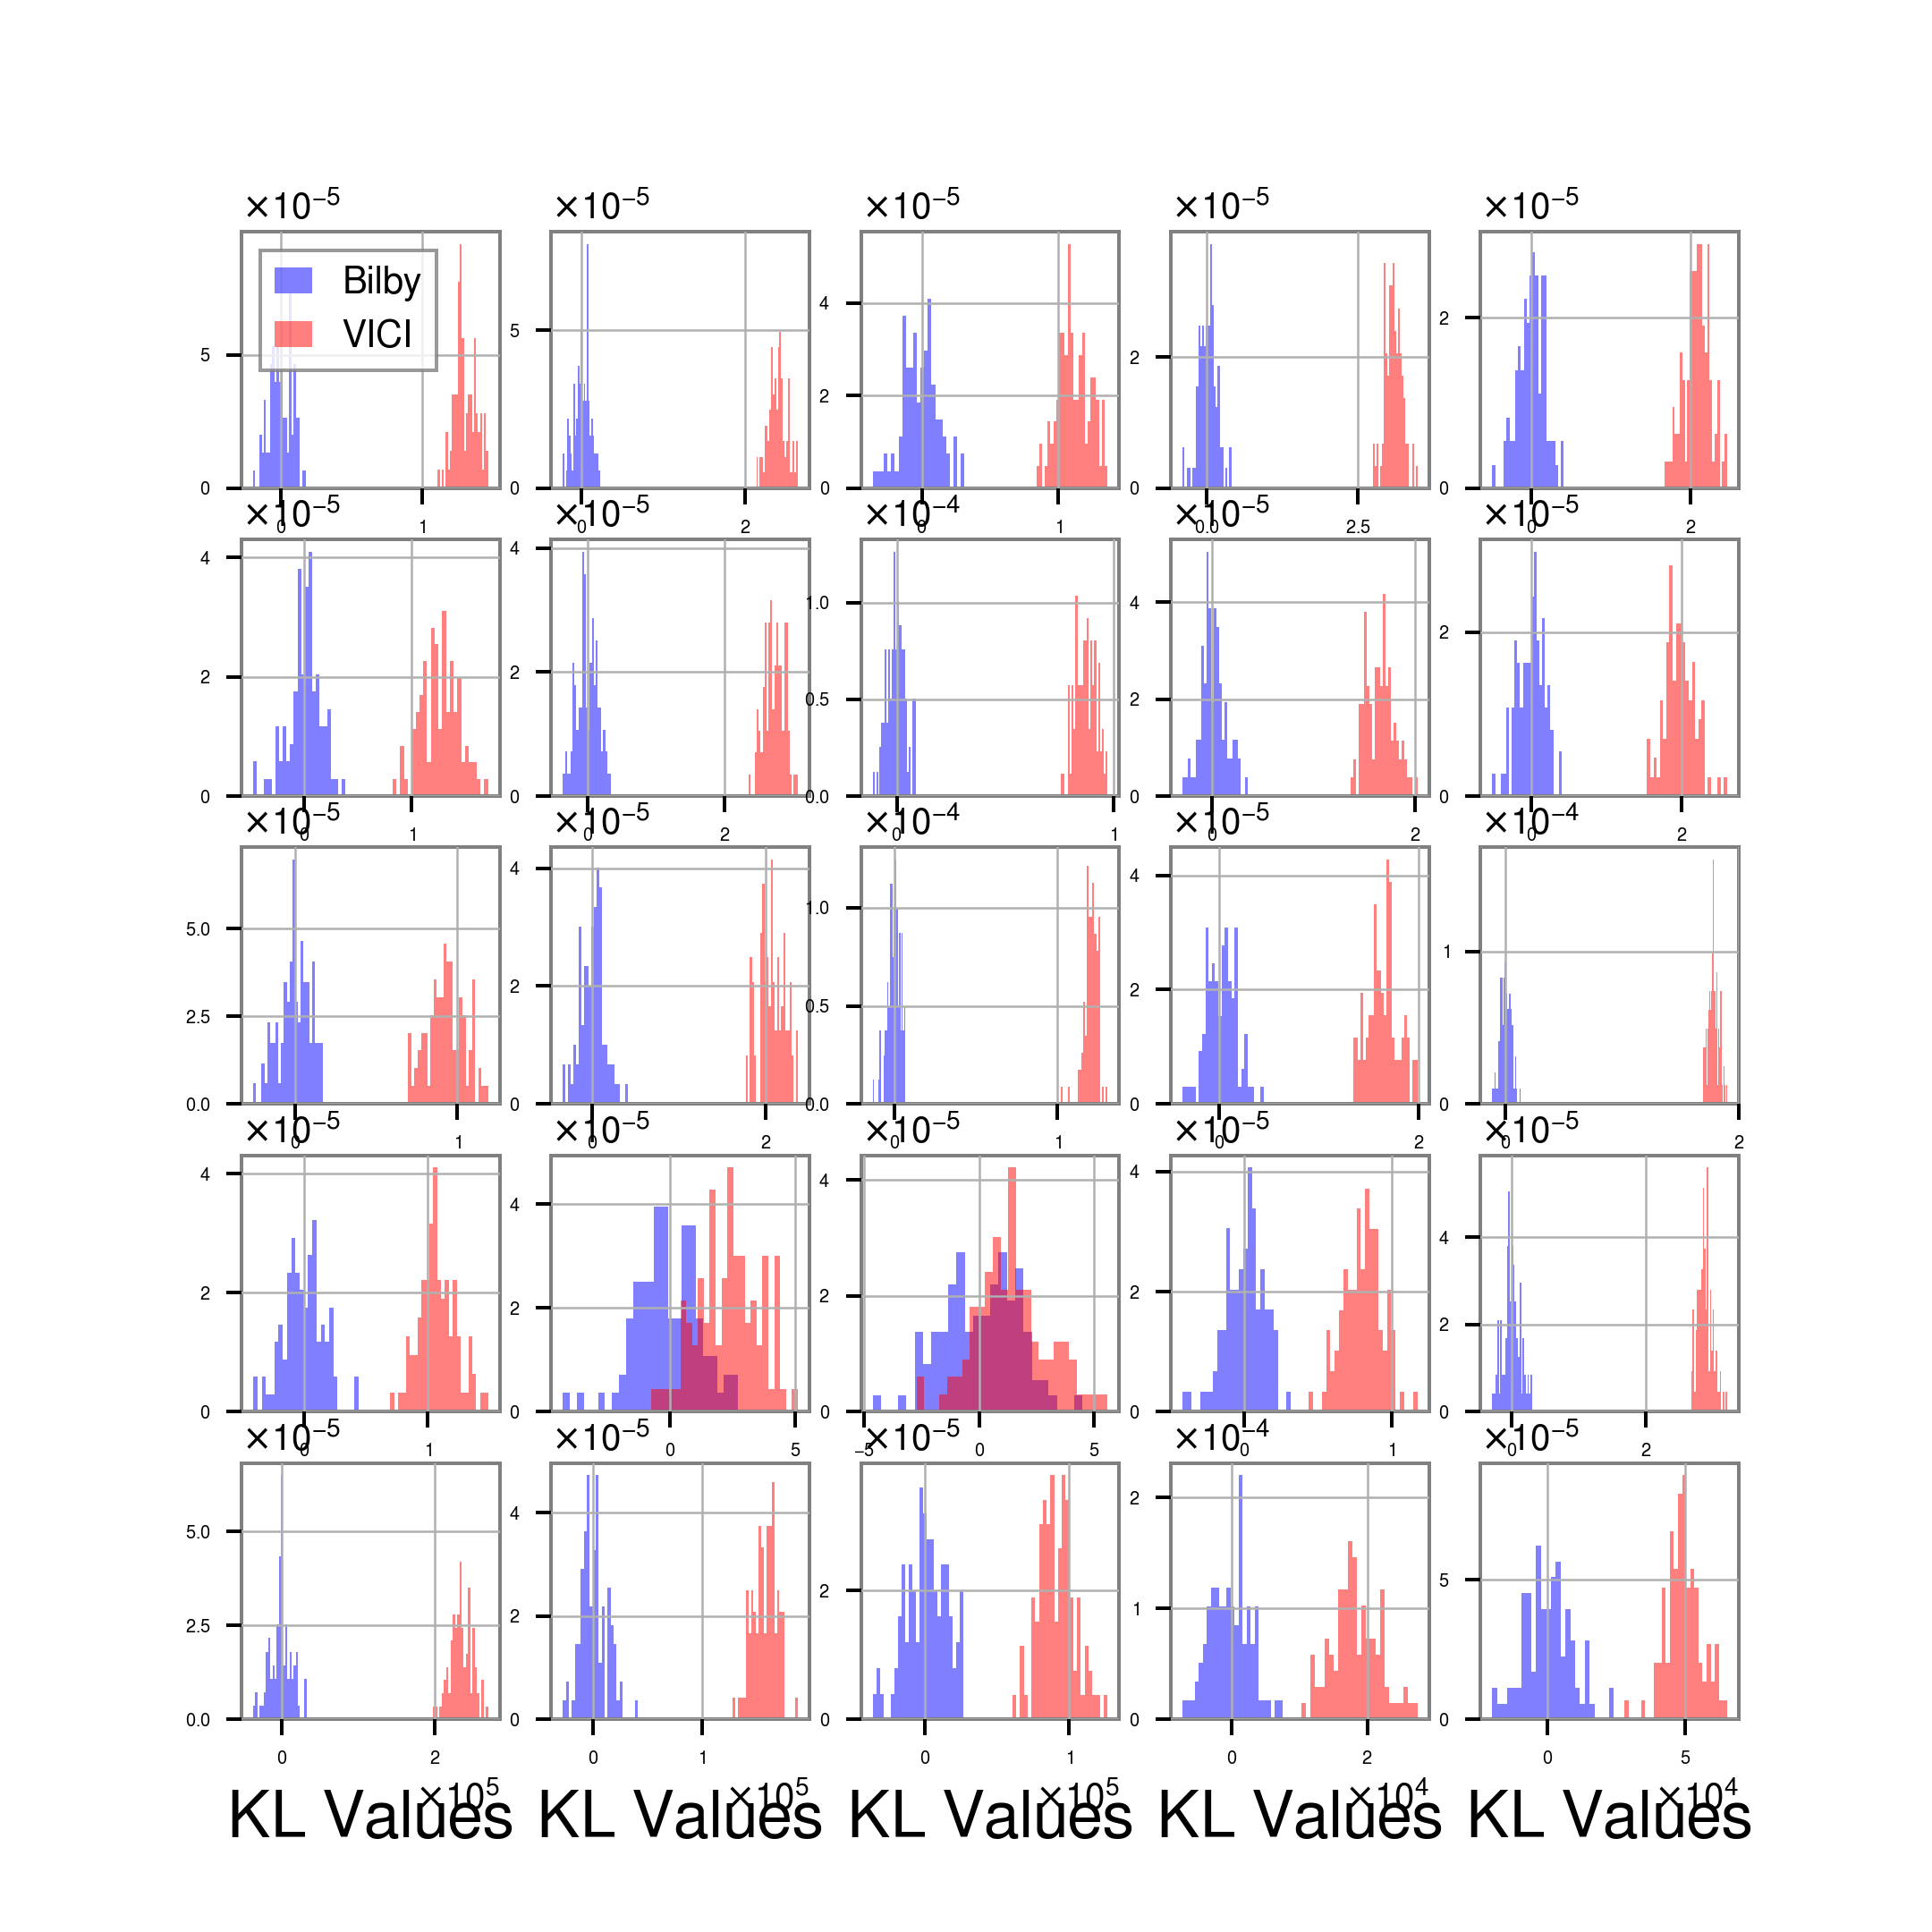
\includegraphics[width=\columnwidth]{images/hist-kl_0.png}
    \caption{\label{fig:kl_results} Histograms of 
    25 different test GW signal KL divergence values. 
    Red denotes predictions from VItamin and blue 
    denotes predictions from Bilby.}
\end{figure}

%
% A-D results
%
\begin{figure}
    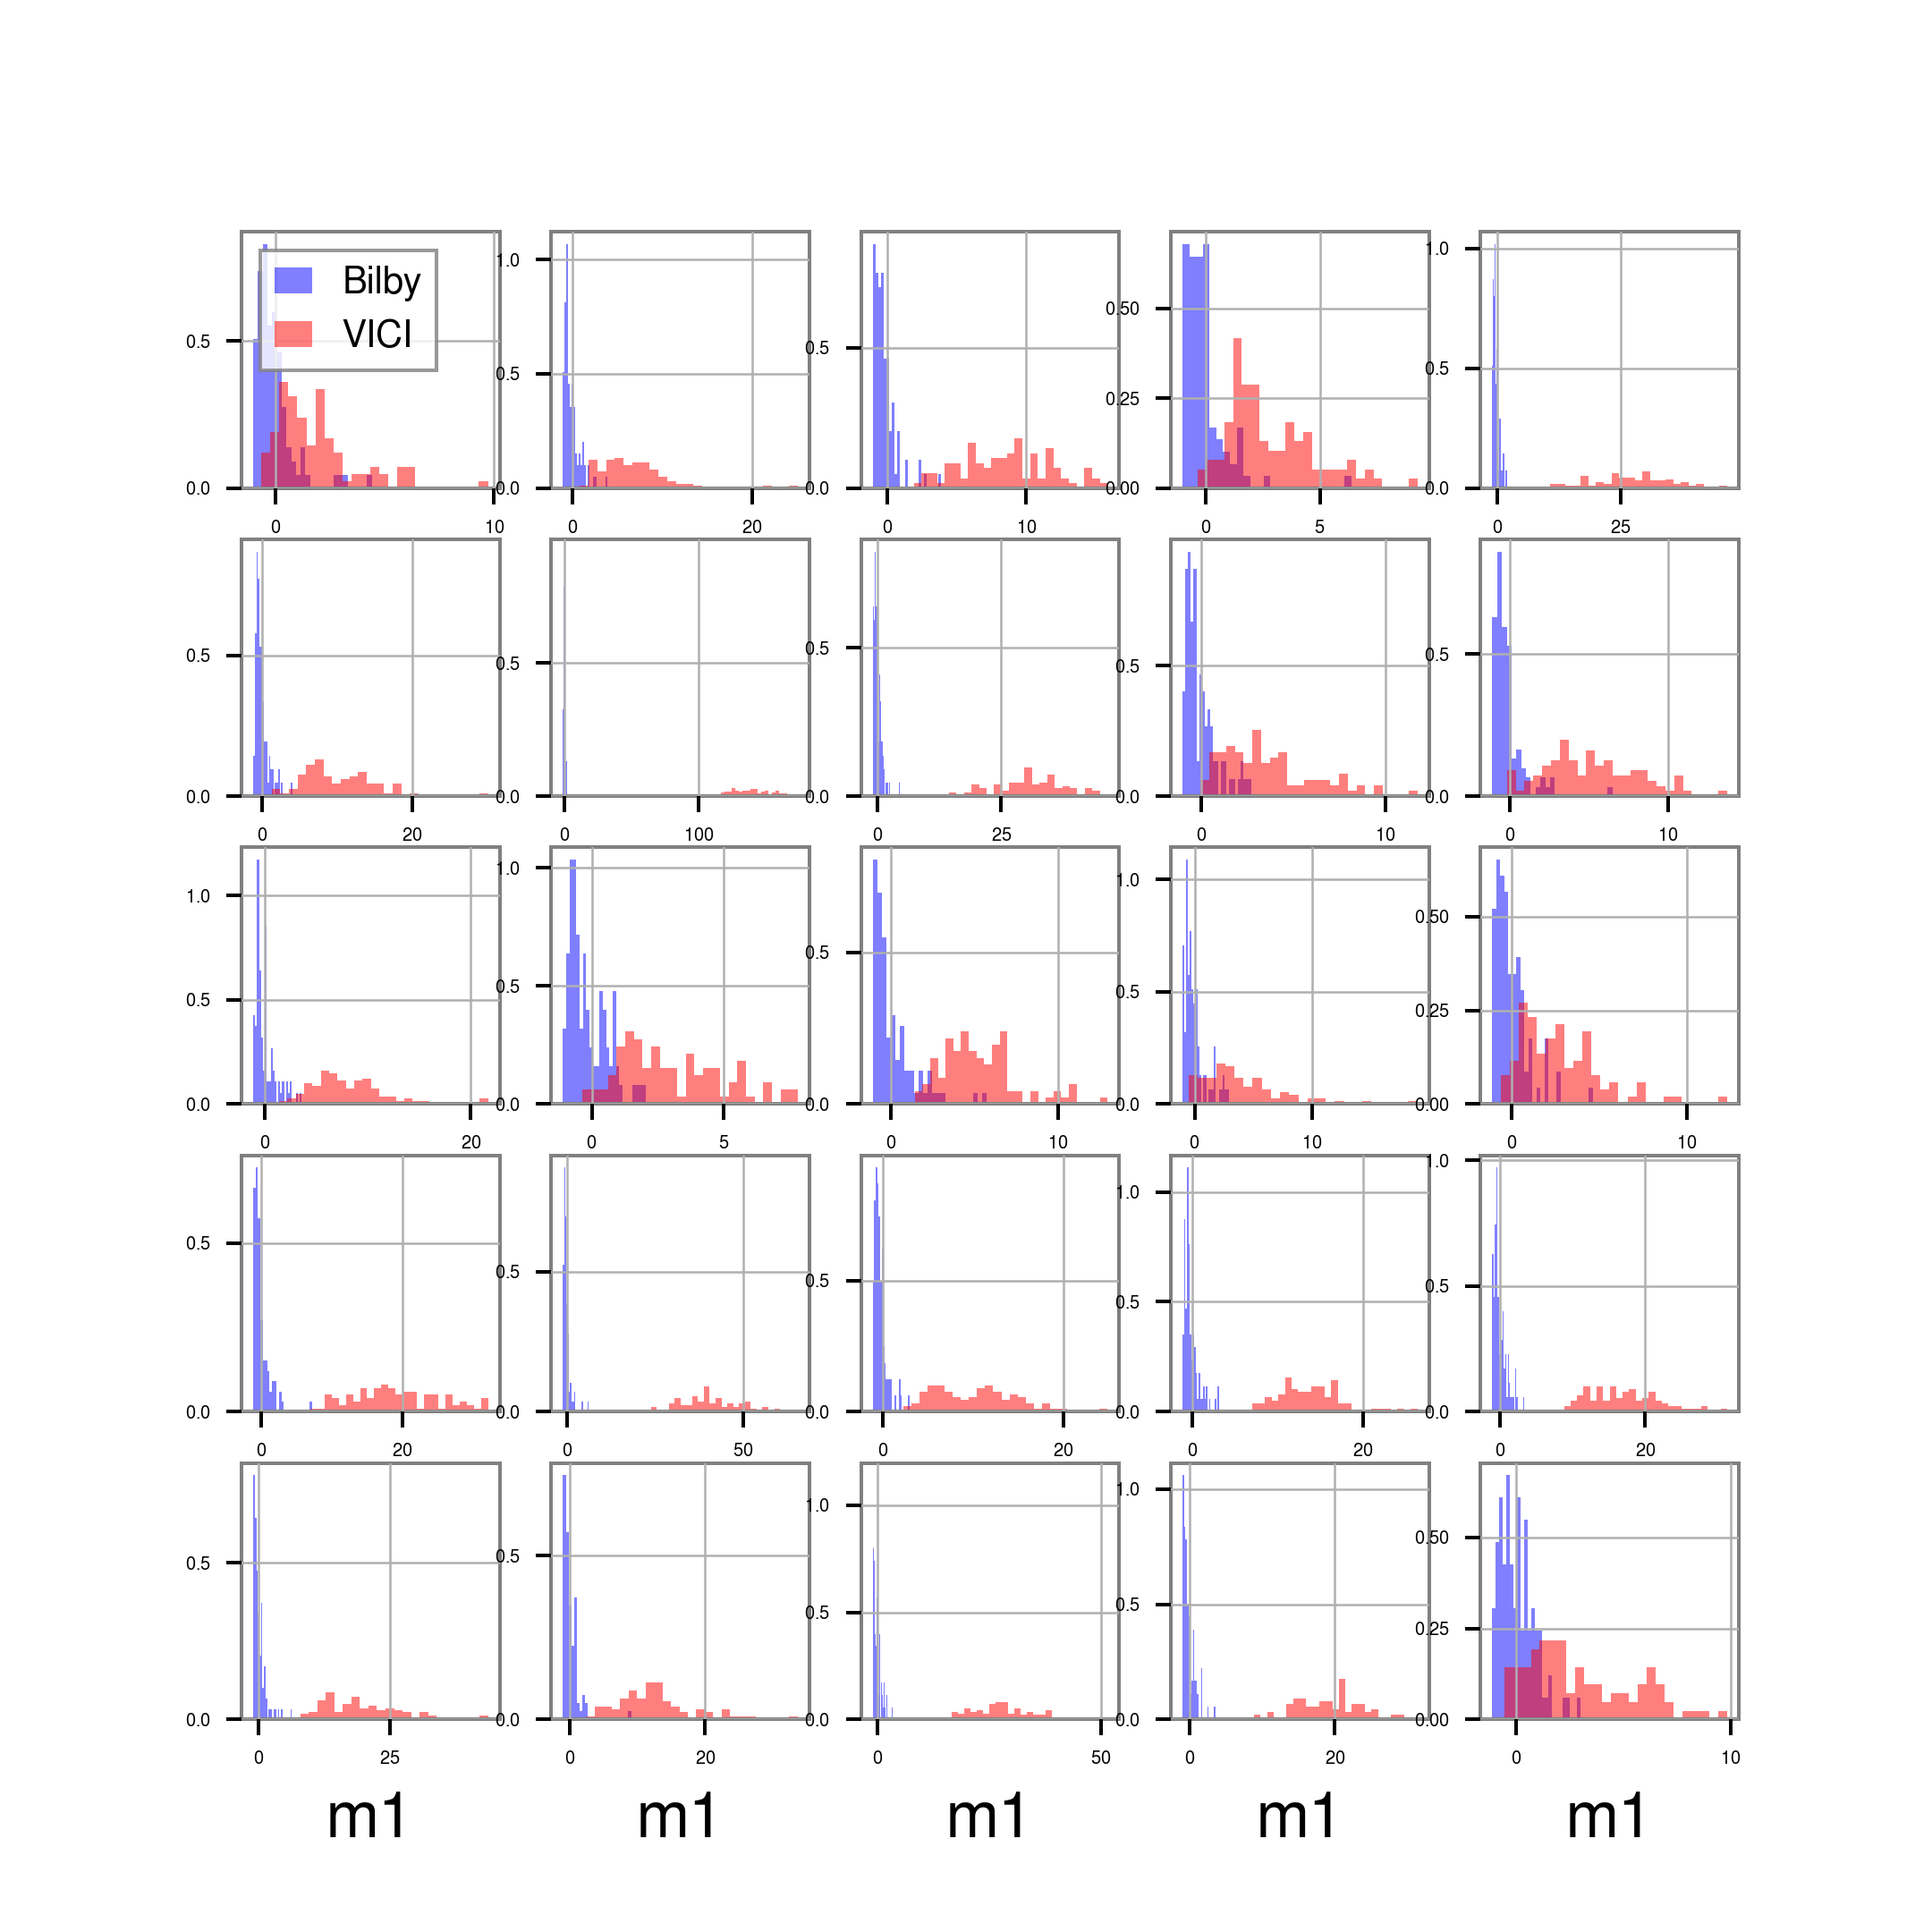
\includegraphics[width=\columnwidth]{images/hist-ad_0.png}
    \caption{\label{fig:ad_results} Histograms of 
    25 different test GW signal Anderson-Darling (AD) statistic 
    component mass 1 values. Distributions which are similar 
    will have AD values which are close to 0.
    Red denotes predictions from VItamin and blue 
    denotes predictions from Bilby.}
\end{figure}

%
% 1-D overlap results
%
\begin{figure}
    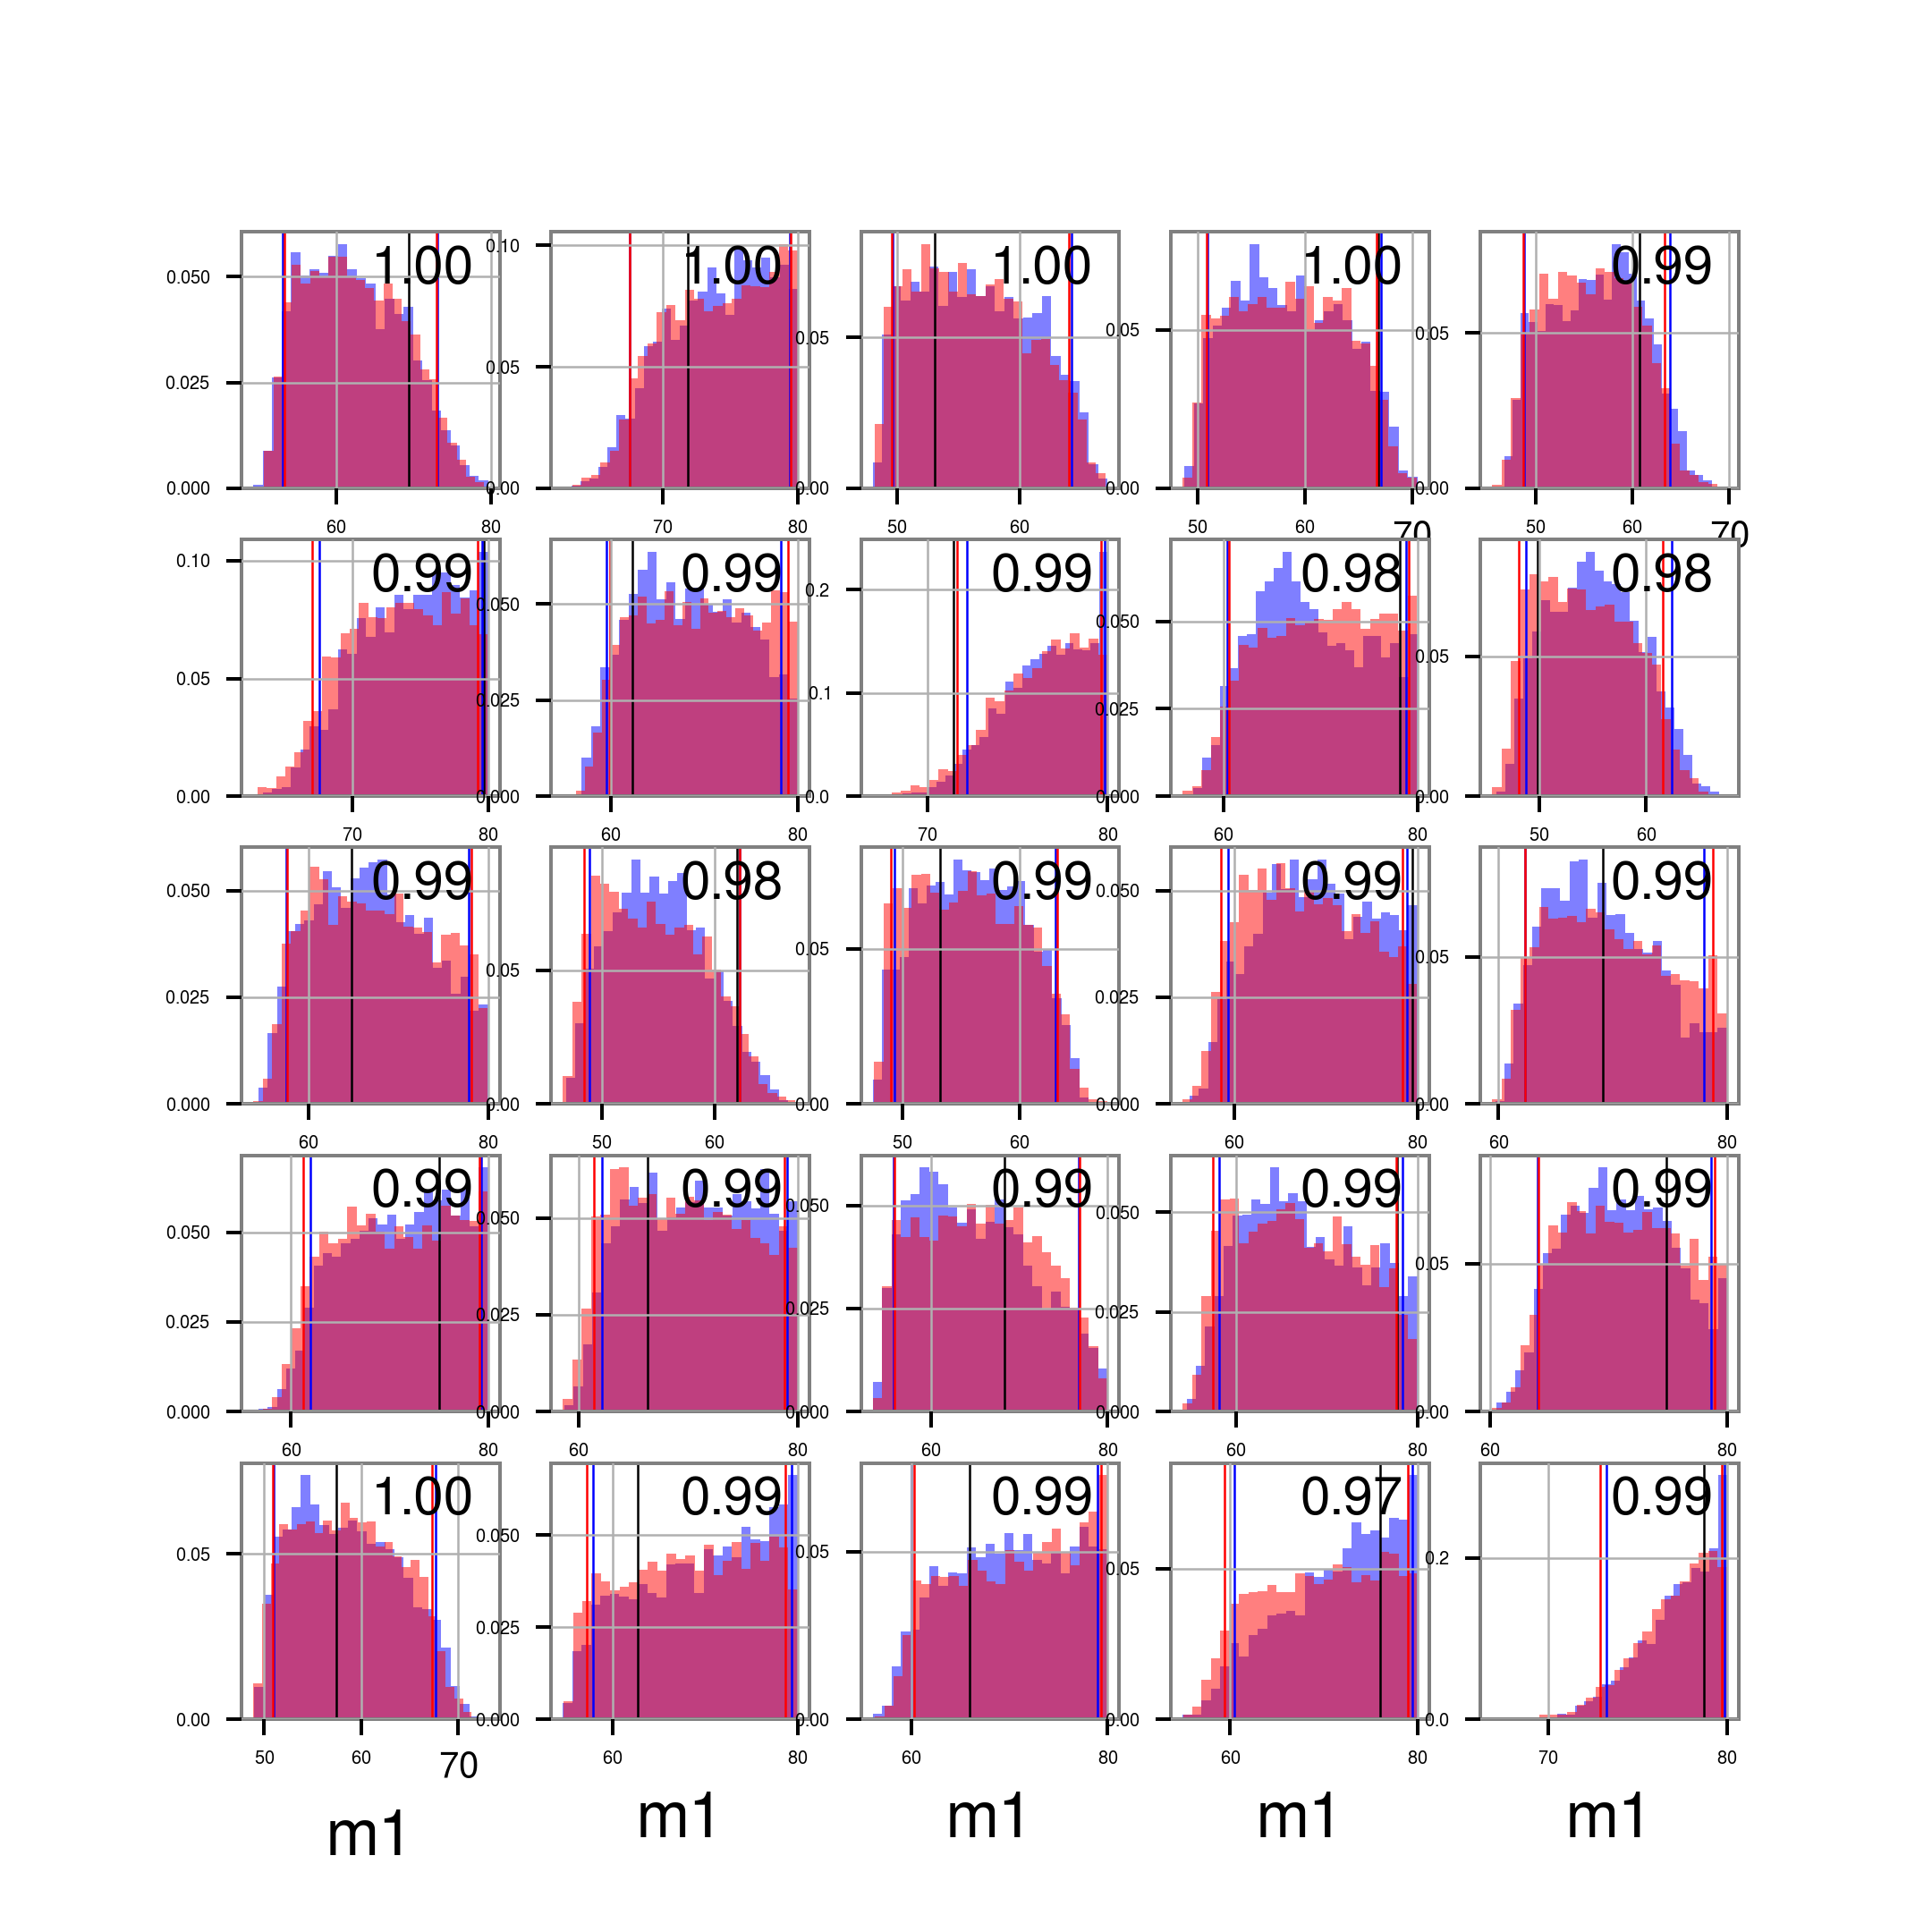
\includegraphics[width=\columnwidth]{images/latest-1d_0.png}
    \caption{\label{fig:1D_overlap} Histograms of 
    25 different test GW signal component mass 1 values. 
    Numbers in the upper right-hand corner denote overlap 
    values where 1 means $\sim{100}\%$ overlap and 0 
    means $\sim{0}\%$ overlap.
    Red denotes predictions from VItamin and blue 
    denotes predictions from Bilby.}
\end{figure}

%
% P-P plot
%
\begin{figure}
    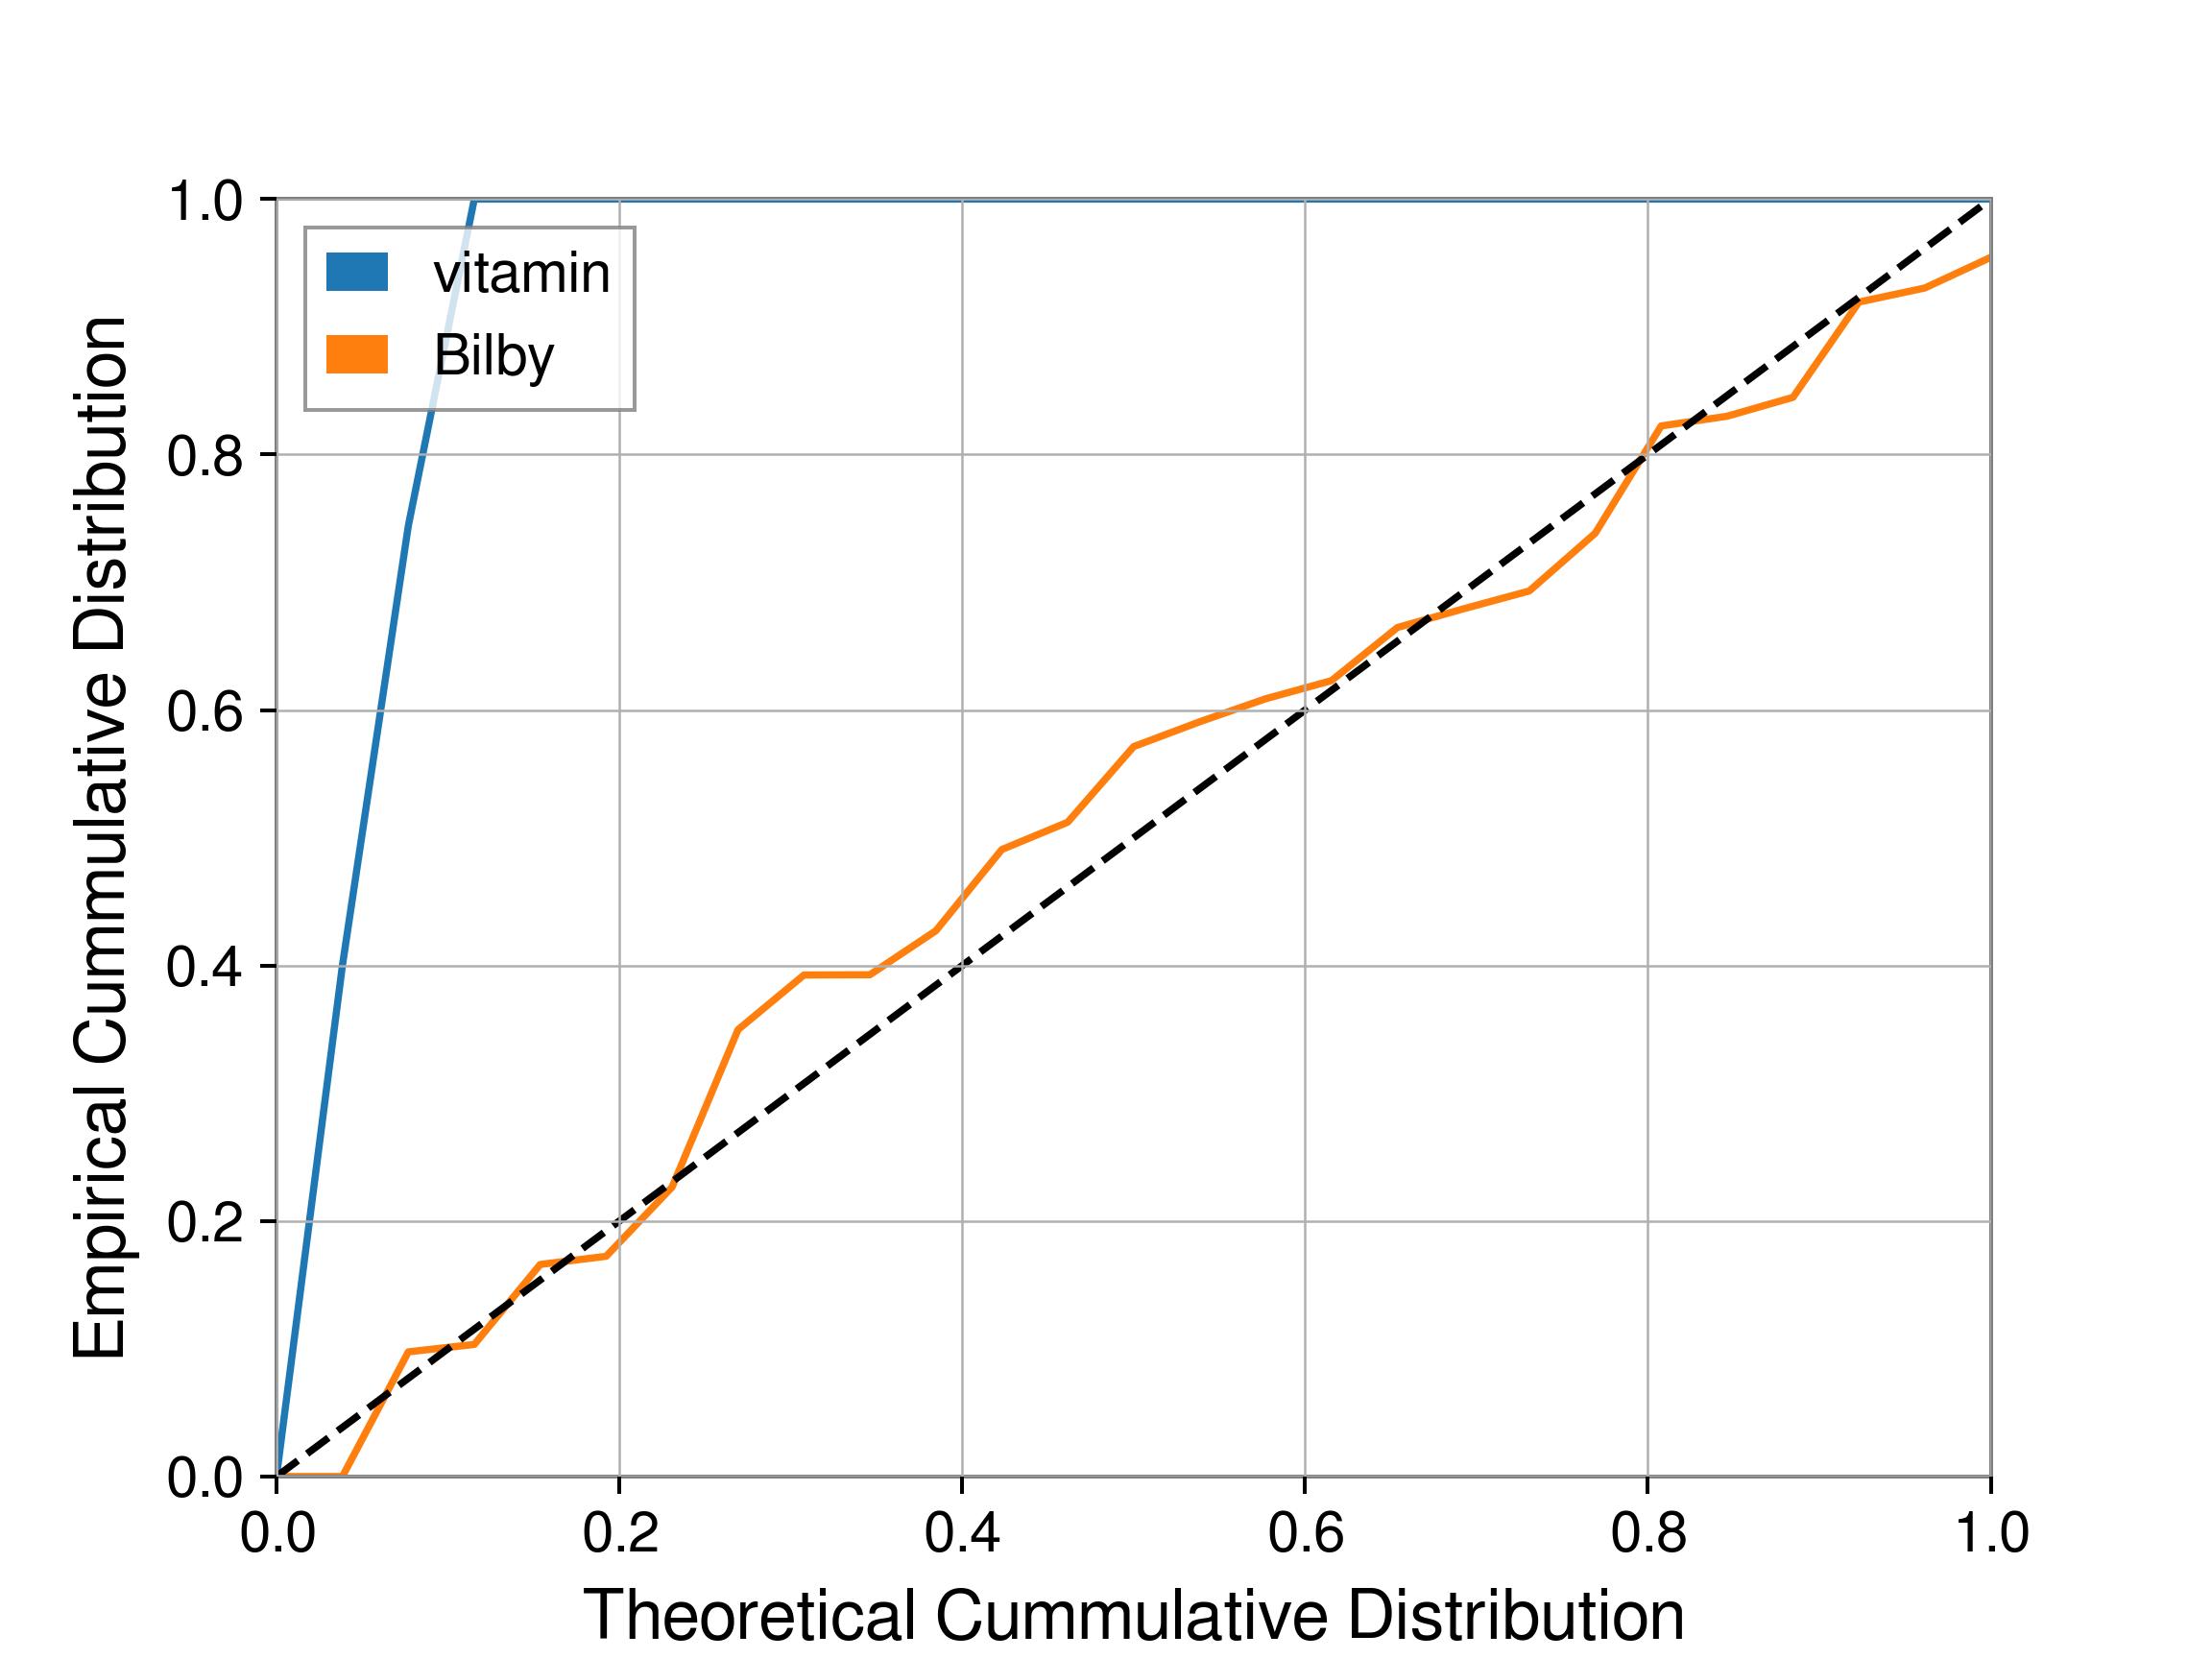
\includegraphics[width=\columnwidth]{images/latest_pp_plot.png}
    \caption{\label{fig:pp_plot} P-p plot 
    using $100$ unique test samples and $5000$
    posterior sample predictions per test sample. 
    The x axis denotes the theoretical cummulative 
    distribution whereas the y axis denotes 
    the predicted cummulative distribution.}
\end{figure}

%
% P-P plot
%
\begin{figure}
    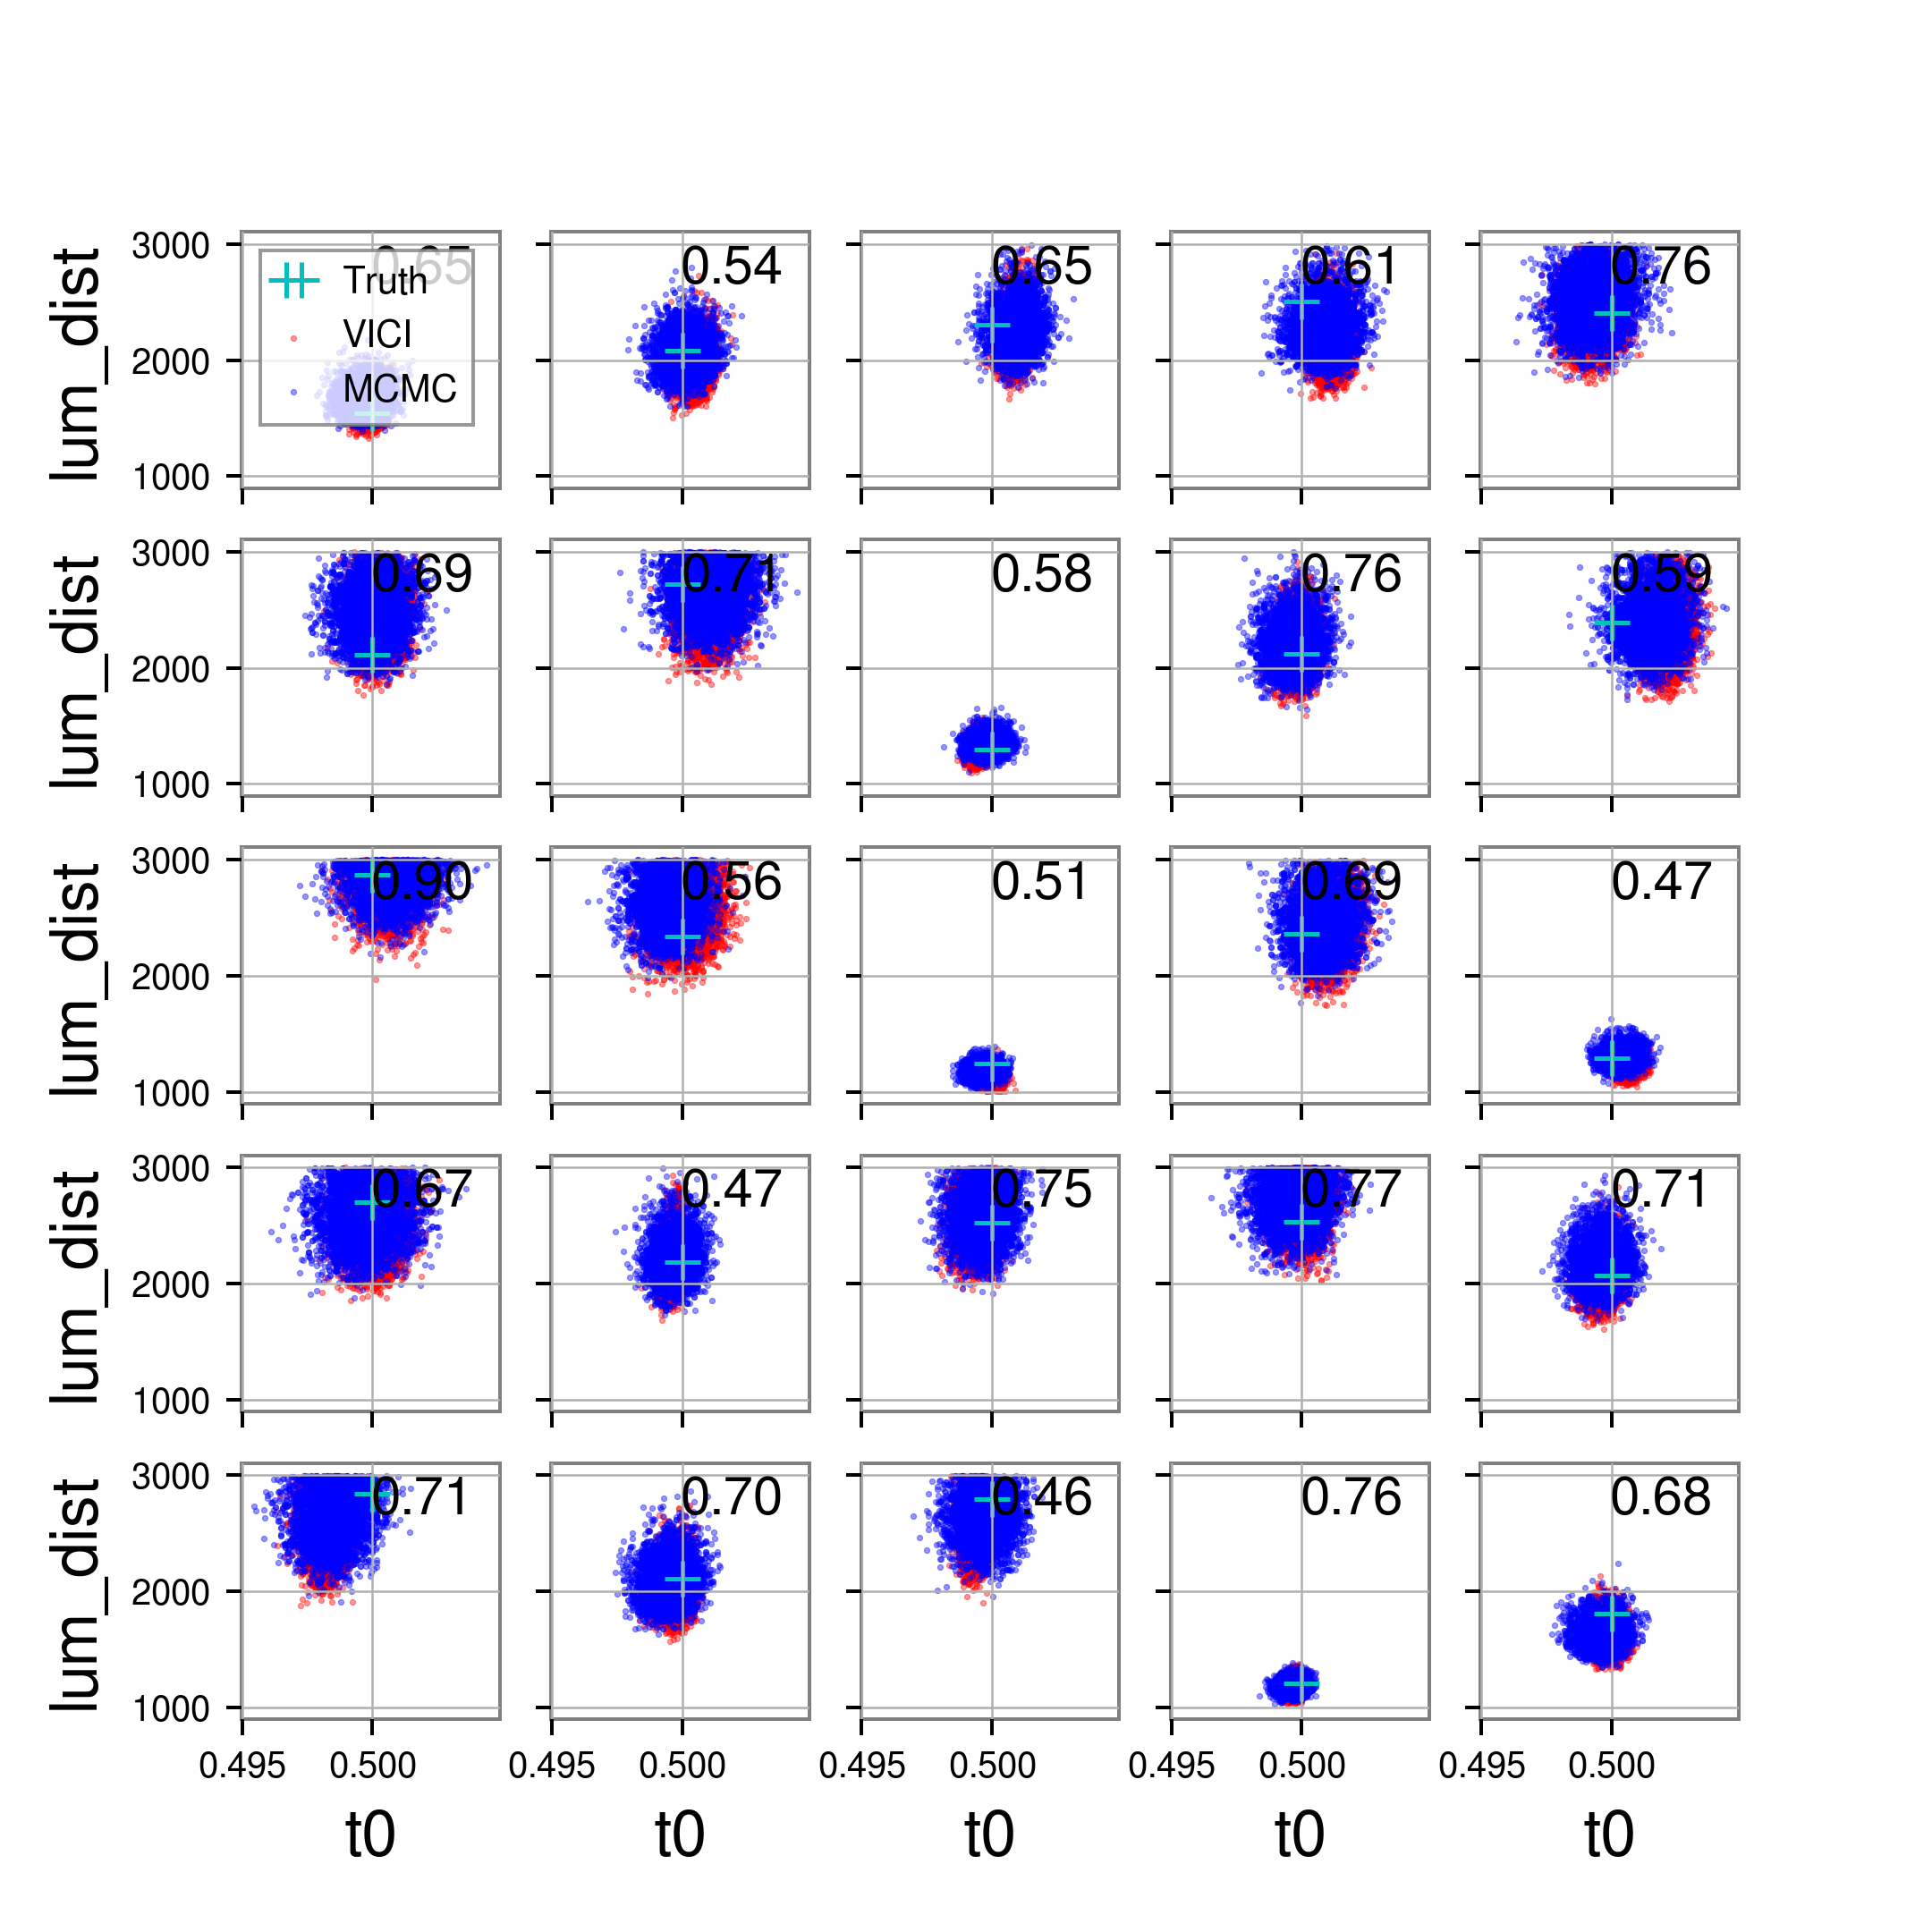
\includegraphics[width=\columnwidth]{images/posteriors_13.png}
    \caption{\label{fig:lum_dist-t0_scatter} This figure illustrates 
    25 different test GW samples with $5000$ posterior samples 
    from both Bilby and VItamin plotted. Red denotes predictions 
    from VItamin and blue denotes predictions from Bilby. Luminosity 
    distance is plotted as a function of time of coalescence.}
\end{figure}

%
% Conclusions
%

\section{Methods}
Put methods in here.  If you are going to subsection it, use
\verb|\subsection| commands.  Methods section should be less than
800 words and if it is less than 200 words, it can be incorporated
into the main text.

\subsection{Method subsection.}

Here is a description of a specific method used.  Note that the
subsection heading ends with a full stop (period) and that the
command is \verb|\subsection{}| not \verb|\subsection*{}|.


%% Put the bibliography here, most people will use BiBTeX in
%% which case the environment below should be replaced with
%% the \bibliography{} command.

% \begin{thebibliography}{1}
% \bibitem{dummy} Articles are restricted to 50 references, Letters
% to 30.
% \bibitem{dummyb} No compound references -- only one source per
% reference.
% \end{thebibliography}

%bibliographystyle{authortitle}
%\bibliography{sample}


%% Here is the endmatter stuff: Supplementary Info, etc.
%% Use \item's to separate, default label is "Acknowledgements"

%\begin{addendum}
% \item Put acknowledgements here.
% \item[Competing Interests] The authors declare that they have no
%competing financial interests.
% \item[Correspondence] Correspondence and requests for materials
%should be addressed to Hunter Gabbard~(email: h.gabbard.1@research.gla.ac.uk).
%\end{addendum}

%%
%% TABLES
%%
%% If there are any tables, put them here.
%%

\begin{table}
\centering
\caption{This is a table with scientific results.}
\medskip
\begin{tabular}{ccccc}
\hline
1 & 2 & 3 & 4 & 5\\
\hline
aaa & bbb & ccc & ddd & eee\\
aaaa & bbbb & cccc & dddd & eeee\\
aaaaa & bbbbb & ccccc & ddddd & eeeee\\
aaaaaa & bbbbbb & cccccc & dddddd & eeeeee\\
1.000 & 2.000 & 3.000 & 4.000 & 5.000\\
\hline
\end{tabular}
\end{table}

\bibliographystyle{apsrev4-1}
\bibliography{references}% Produces the bibliography via BibTeX.

\end{document}
